\chapter{Method}\label{chapter:first_real_chapter}

Our method is based on an Hiearchical VAE (H-VAE), as these have been shown to improve the sharpness of the resulting generated sample. There are 3 submodels present, the image encoder $p_\theta(x | z)$\footnote[1]{$z$ will consist of multiple layers as it is an H-VAE. Sometimes denoted as $z_{1:L}$.}, the image decoder $q_\phi(z | x)$\footnotemark[1] and the label decoder $q_\xi(z | y)$\footnotemark[1]. The image encoder and decoder can be pretrained on unlabeled data. Subsequently the label decoder will be trained from the (variational) latent variables, on a subset of the inital dataset $\mathcal{D}$.

\begin{figure}[h]
    \begin{minipage}{0.45\textwidth}
        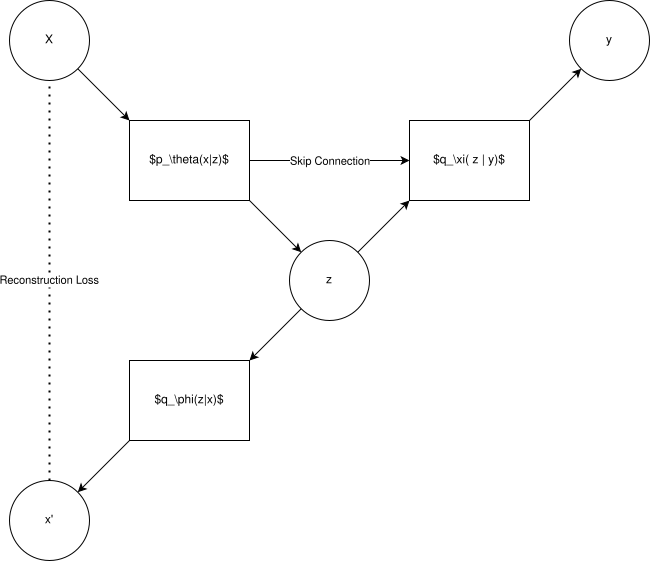
\includegraphics[width=1\textwidth]{figures/model_data_flow.png}
        \caption{The data flow of the various submodels.}
    \end{minipage}
    \hfill
    \begin{minipage}{0.45\textwidth}
        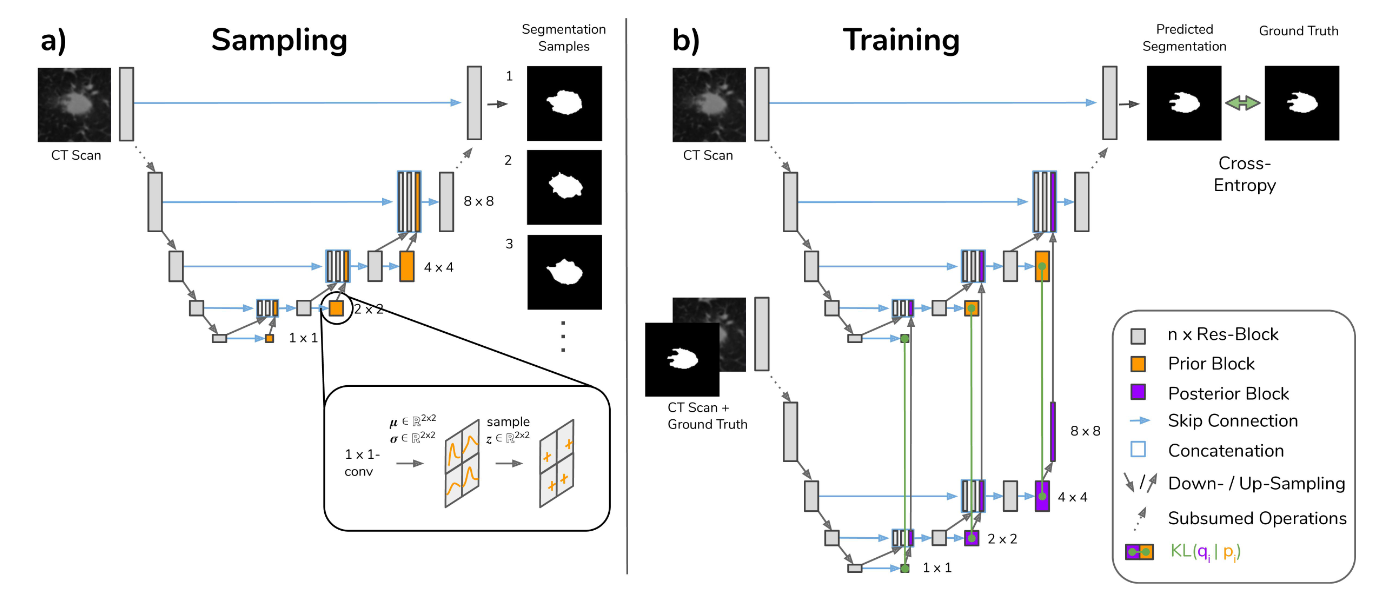
\includegraphics[width=1\textwidth]{figures/h_vae_structure.png}
        \caption{Example of the H-VAE structure. From \cite{kohl2018probabilistic}. This does not include the pretraining of the encoder.}
    \end{minipage}
\end{figure}

\subsection*{Why VAE?}
By using a VAE bootstrapping can be applied during inference to provide an insight in the certainty of the model, as has been shown by \cite{kohl2018probabilistic}. This certainty estimation from the bootstrapping is crucial in mobile robotics and can be done quickly using batched inference.

